%
% No cal saber gaire LaTeX per escriure una tesi.
%
% Afegiu el vostre text a la plantilla, i deixeu que Knuth i
% Lamport s'encarreguin de l'aspecte.

% Per crear el document en .pdf només cal fer 'pdflatex
% aquestarxiu.tex', 'bibtex aquestarxiu' (sense extensió) i
% 'pdflatex aquestarxiu.tex' un altre cop. Hi ha moltes eines que
% permeten simplificar moltíssim la compilació en latex (v, p.ex.,
% rubber: http://www.pps.jussieu.fr/~beffara/soft/rubber/)
%

% [ Tots els caràcters que segueixen el signe %, fins a final de
%   línia, són comentaris i no es processen. ]
%
% En el bloc següent, delimitat per dues línies d'asteriscs,
% s'especifica el format del document. El podeu ignorar sense
% problemes si no sabeu LaTeX.
%

% *****************************************************************************

% Aquí s'especifica quin tipus de document voleu, i quines
% extensions (llengua, gràfics, fonts) fareu servir.

\RequirePackage{fix-cm}                 % Technicalities
\documentclass[10pt,b5paper,twoside,showtrims,openright]{memoir}
\usepackage[utf8]{inputenc} 		% codificació dels caràcters
\usepackage[catalan,english]{babel}	% localització de l'estil
\usepackage{url}			% macro \url per introduir adreces
\usepackage{amsmath}			% macros per matemàtiques
\usepackage{amssymb}			% macros per matemàtiques
\usepackage{amsfonts}			% macros per matemàtiques
\usepackage[pdftex]{graphicx}		% suport per figures
\usepackage{color}                      % per poder fer servir colors
\usepackage[colorlinks,bookmarks,pdftex,hyperfigures,breaklinks]{hyperref} % produeix enllaços clicables
\usepackage[T1]{fontenc}                % Nou esquema de codificació (recomanat)
\usepackage[round,authoryear]{natbib}  % per poder fer citacions Autor-any
%\usepackage{fixltx2e}                   % Technicalities

\DeclareGraphicsExtensions{.pdf,.png} % preference order

\hypersetup{
    pdfauthor={David García Garzón},
    pdftitle={PhD Thesis: TODO},
}
%% Format UPF, dues cares.
% Recordeu que les dimensions d'A4 i B5 són (210mm,297mm) i
% (176mm,250mm), respectivament.


\setulmarginsandblock{30mm}{*}{1.0}  % Marges verticals (3cm a dalt, 1.0*3cm a baix)
\setlrmarginsandblock{*}{30mm}{1.0} % Marges laterals (3cm a la dreta, 1.0*3cm l'esquerra)



% Per defecte la classe 'memoir' no numera les subseccions. Que les numeri:
\maxsecnumdepth{subsection}
\setsecnumdepth{subsection}
% Tampoc no inclou les subseccions a l'Índex. Que les inclogui:
\maxtocdepth{subsection}
\settocdepth{subsection}

% Estil dels capítols (consulteu estils disponibles a
% http://www.imf.au.dk/system/latex/artikler/MemoirChapStyles/MemoirChapStyles.pdf)
\chapterstyle{hangnum}

% Colors dels enllaços clickables (els que hi ha per defecte són molt
% kitsch)
\definecolor{LinkColor}{rgb}{0, 0, 0.3}
\definecolor{ExtLinkColor}{rgb}{0, 0.3, 0}
\hypersetup{citecolor=LinkColor,linkcolor=LinkColor,urlcolor=ExtLinkColor}


% **********************************************************************************

%%%%%%%%%%%%%%%%%%%%%%%%%%%%%%%%%%%%%%%%%%%%%%%%%%%%%%%%%%%%%%%%%%%%%%%%%%
%%%%%%%%%%%%%%%%%%%%%%%%%% Macros %%%%%%%%%%%%%%%%%%%%%%%%%%%%%%%%%%%%%%%%
%%%%%%%%%%%%%%%%%%%%%%%%%%%%%%%%%%%%%%%%%%%%%%%%%%%%%%%%%%%%%%%%%%%%%%%%%%

%%%%%%%%%%%%%%%%%%%%%%%% Structure definitions %%%%%%%%%%%%%%%%%%%%%%%%%%%

\newcommand{\bref}[1]{(\ref{#1})}

\newcommand{\eqn}[1]{(\ref{#1})}
\newcommand{\be}{\begin{equation}}
\newcommand{\ee}{\end{equation}}
\newcommand{\ben}{\begin{displaymath}}
\newcommand{\een}{\end{displaymath}}
\newcommand{\bea}{\begin{eqnarray}}
\newcommand{\eea}{\end{eqnarray}}
\newcommand{\bean}{\begin{eqnarray*}}
\newcommand{\eean}{\end{eqnarray*}}
\newcommand{\nn}{\nonumber \\}
\newcommand{\ba}{\begin{array}}
\newcommand{\ea}{\end{array}}
\newcommand{\bi}{\begin{itemize}}
\newcommand{\ei}{\end{itemize}}

%some of Rob's additions
\newcommand{\labell}[1]{\label{#1}\qquad_{#1}} %{\label{#1}}
\newcommand{\reef}[1]{(\ref{#1})}
\newcommand{\non}{\nonumber}
\newcommand{\pf}{\partial}
\newcommand{\bZ}{\bar{Z}}
\newcommand{\dZ}{\dot{Z}}
\newcommand{\dr}{\dot{r}}
\newcommand{\dbZ}{\dot{\bZ}}
\newcommand{\bz}{\bar{z}}
\newcommand{\dz}{\dot{z}}
\newcommand{\dbz}{\dot{\bz}}
\newcommand{\dU}{U^\dagger}
\def\cc{\mathbb{C}}
\newcommand{\df}{\textrm{d}}
%\newcommand{\str}{{\rm STr}}
%\newcommand{\tr}{{\rm Tr}}
\newcommand{\tr}{\mbox{Tr}}
\newcommand{\str}{\mbox{str}}

\newcommand{\mt}[1]{\textrm{\tiny #1}}
\def\lt {\lambda}
\def\rt {r}
\def\rhot {\rho}
\def \rvac{r_\mt{vac}}
\def\nc {N_\mt{c}}
\def\nf {N_\mt{f}}
\def\ua {U(1)_\mt{A}}
\def\tsix {T_\mt{D6}}
\def\ut {U_\mt{KK}}
\def\uh {U_\mt{T}}
\def\gym {g_\mt{YM}}
\newcommand{\nonsol}{D4-soliton}
\newcommand{\te}{t_\mt{E}}
\newcommand{\ct}{T_\mt{deconf}}
\newcommand{\tcc}{T_\mt{fund}}
\newcommand{\tb}{\bar{M}}
\newcommand{\msusy}{M_\mt{susy}}
\newcommand{\lm}{\l_\mt{match}}

\def\l{\lambda}
\def\a{\alpha}
\def\ap{\alpha'}
\def\b{\beta}
\def\g{\gamma}
\def\bg{\bar{\gamma}}
\def\G{\Gamma}
\def\d{\delta}
\def\s{\sigma}
\def\e{\epsilon}
\def\vt{\vartheta}
\def\vp{\varphi}
\def\T{\Theta}
\def\u{u}
%Introduced by Toni:

\def\otaula{\begin{tabular}}
\def\ctaula{\end{tabular}}


\renewcommand{\O}{\Omega}
\renewcommand{\L}{\Lambda}
\renewcommand{\t}{\theta}
%\renewcommand{\om}{\omega}



% Shortcuts added by Toni:

\def\bnum{\begin{enumerate}}
\def\enum{\end{enumerate}}
\newcommand{\num}[1]{\enub {#1} \enue}

\def\CR{\mathbb{R}}
\def\CM{\mathcal{M}}
\def\CC{\mathcal{C}}
\def\CE{\mathcal{E}}
\def\CQ{\mathcal{Q}}
\def\avall{\vskip 0.3cm}
\def\espai{\;\;\;\;\;\;\;}
\def\zespai{\;\;\;\;}
\def\s{\sigma}
\def\8M{$\CM_8$}
\def\k{\kappa}
\def\be{\begin{equation}}
\def\ee{\end{equation}}
\def\G{\Gamma}
\def\g{\gamma}
\def\ei{e^{\underline{i}}}
\def\ej{e^{\underline{j}}}
\def\e1{e^{\underline{1}}}
\def\1u{\underline{1}}
\def\2u{\underline{2}}
\def\iu{\underline{i}}
\def\0u{\underline{0}}
\def\e{\epsilon}
\def\target{$\CR^{1,1}\times \mathcal{M}_8$ }
\def\target2{$\CR^{1,1}\times \mathcal{M}_8$,}
\def\9G{\G_{\underline{9}}}
%\def\otaula{\begin{tabular}}
%\def\ctaula{\end{tabular}}
\def\yvec{\vec{y}}
\def\kvec{\vec{k}}
\def\rvec{\vec{r}}
\def\xvec{\vec{x}}

\def\a{\alpha}
\def\b{\beta}
\def\undos{{1\over 2}}
\def\p{\partial}
\def\we{\wedge}

\def\xespai{\,, \zespai}

\def\tl{\tilde{L}}
\def\ads{$AdS_5 \times S^5$ }
\def\kap{$\kappa$-symmetry }
\def\tg{\tilde{\gamma}}

%%%%%%%%%%%%%%%%%% Calligraphic Letters %%%%%%%%%%%%%%%%%%%%%%%%%%%%%%%%%

\newcommand{\cala}{\mbox{${\mathcal A}$}}
\newcommand{\calb}{\mbox{${\mathcal B}$}}
\newcommand{\calc}{\mbox{${\mathcal C}$}}
\newcommand{\cald}{\mbox{${\mathcal D}$}}
\newcommand{\cale}{\mbox{${\mathcal E}$}}
\newcommand{\calf}{\mbox{${\mathcal F}$}}
\newcommand{\calg}{\mbox{${\mathcal G}$}}
\newcommand{\calh}{\mbox{${\mathcal H}$}}
\newcommand{\cali}{\mbox{${\mathcal I}$}}
\newcommand{\calj}{\mbox{${\mathcal J}$}}
\newcommand{\calk}{\mbox{${\mathcal K}$}}
\newcommand{\call}{\mbox{${\mathcal L}$}}
\newcommand{\calm}{\mbox{${\mathcal M}$}}
\newcommand{\caln}{\mbox{${\mathcal N}$}}
\newcommand{\calo}{\mbox{${\mathcal O}$}}
\newcommand{\calp}{\mbox{${\mathcal P}$}}
\newcommand{\calq}{\mbox{${\mathcal Q}$}}
\newcommand{\calr}{\mbox{${\mathcal R}$}}
\newcommand{\cals}{\mbox{${\mathcal S}$}}
\newcommand{\calt}{\mbox{${\mathcal T}$}}
\newcommand{\calu}{\mbox{${\mathcal U}$}}
\newcommand{\calv}{\mbox{${\mathcal V}$}}
\newcommand{\calw}{\mbox{${\mathcal W}$}}
\newcommand{\calx}{\mbox{${\mathcal X}$}}
\newcommand{\caly}{\mbox{${\mathcal Y}$}}
\newcommand{\calz}{\mbox{${\mathcal Z}$}}

\newcommand{\bfcalc}{\mbox{\boldmath ${\cal C}$}}


%%%%%%%%%%%%%%%%% Boldmath Letters %%%%%%%%%%%%%%%%%%%%%%%%%%%%%%%%%%%%%%

\newcommand{\bfe}{\mbox{\boldmath $E$}}
\newcommand{\bfb}{\mbox{\boldmath $B$}}
\newcommand{\bfpi}{\mbox{\boldmath $\Pi$}}
\newcommand{\bfp}{\mbox{\boldmath $P$}}
\newcommand{\bfna}{\mbox{\boldmath $\nabla$}}
\newcommand{\bfd}{\mbox{\boldmath $D$}}
\newcommand{\bfeh}{\mbox{\boldmath $\hat{E}$}}
\newcommand{\bfbh}{\mbox{\boldmath $\hat{B}$}}
\newcommand{\bfah}{\mbox{\boldmath $\hat{A}$}}
\newcommand{\bx}{\mbox{\boldmath $x$}}
\newcommand{\by}{\mbox{\boldmath $y$}}
\newcommand{\bX}{\mbox{\boldmath $X$}}
\newcommand{\bY}{\mbox{\boldmath $Y$}}
\newcommand{\bV}{\mbox{\boldmath $V$}}
\newcommand{\bU}{\mbox{\boldmath $U$}}

\newcommand{\bfK}{\mbox{\boldmath $K$}}
\newcommand{\bfz}{\mbox{\boldmath $\theta$}}
\newcommand{\bfZ}{\mbox{\boldmath $Z$}}
\newcommand{\bfr}{\mbox{\boldmath $\rho$}}
\newcommand{\bfxi}{\mbox{\boldmath $\xi$}}
\newcommand{\bfs}{\mbox{\boldmath $\sigma$}}
\newcommand{\bft}{\mbox{\boldmath $t$}}
\newcommand{\bfT}{\mbox{\boldmath $T$}}
\newcommand{\bfss}{\mbox{\boldmath $s$}}
\newcommand{\bfS}{\mbox{\boldmath $S$}}
\newcommand{\bfG}{\mbox{\boldmath $\Gamma$}}
\newcommand{\bfo}{\mbox{\boldmath $0$}}

\newcommand{\bbe}[1]{\mbox{${\mathbb E}^{#1}$}}
\newcommand{\bbr}[1]{\mbox{${\mathbb R}^{#1}$}}
%\newcommand{\bbz}[1]{\mbox{${\mathbb Z}^{#1}$}}
\newcommand{\bbz}[1]{\mbox{${\mathbb Z}_{#1}$}}
\newcommand{\bbi}[1]{\mbox{${\mathbb I}_{#1}$}}
\newcommand{\bbo}[1]{\mbox{${\mathbb O}_{#1}$}}

%%%%%%%%%%%%%%%%%%%%%% Miscellaneous  %%%%%%%%%%%%%%%%%%%%%%%%%%%%%%%%%%%

\newcommand{\nef}{{$\caln =4$} }

\newcommand{\dd}[3]{\mbox{$( #1 | \mbox{D} #2 \perp \mbox{D} #3)$}}
\newcommand{\ds}[3]{\mbox{$( #1 | D #2 \perp \calt #3)$}}
\newcommand{\para}{\parallel}
\newcommand{\inter}{\, \cap \,}
\newcommand{\su}[1]{$\calt #1\,$}

\newcommand{\adss}[2]{\mbox{$AdS_{#1}\times {S}^{#2}$}}
\newcommand{\rn}{Reissner-Nordstr\"{o}m }

\newcommand{\bra}[1]{\mbox{$\langle #1 |$}}
\newcommand{\ket}[1]{\mbox{$| #1 \rangle$}}
\newcommand{\braket}[2]{\mbox{$\langle #1  | #2 \rangle$}}
\newcommand{\proj}[1]{\ket{#1}\!\bra{#1}}

\newcommand{\Gu}[1]{\Gamma_{\underline{#1}}}
\newcommand{\Gn}{\Gamma_\natural}

\newcommand{\un}{\underline}
\newcommand{\pa}{\partial}
\newcommand{\fc}{\frac}
\newcommand{\trace}{\mbox{Tr}}
\newcommand{\sac}{\, , \qquad}
%\newcommand{\eg}{{\it e.g. }}
%\newcommand{\ie}{{\it i.e. }}
\newcommand{\sgn}[1]{\mbox{sgn}(#1)}
\newcommand{\com}[1]{[[[{\bf #1}]]]}
\newcommand{\ad}{\dot{a}}
\newcommand{\bd}{\dot{b}}
\newcommand{\ik}{{\it k}}
\newcommand{\ione}{{\it 1}}
\newcommand{\itwo}{{\it 2}}
\newcommand{\ifive}{{\it 5}}

\newcommand{\ph}{\hat{P}}
\newcommand{\xh}{\hat{X}}
\newcommand{\ve}{\varepsilon}


\newcommand{\ra}{\rightarrow}

\newcommand{\ignore}[1]{}

%%%%%%%%%%%%%%%%%%%%%%%%%%% For This %%%%%%%%%%%%%%%%%%%%%%%
\def\pamu{\partial_{\mu}}
\def\spamu{\partial^{\mu}}
\def\spanu{\partial^{\nu}}
\def\panu{\partial_{\nu}}
\def\pasi{\partial_{\sigma}}
\def\parho{\partial_{\rho}}
\def\Udag{U^{\dagger}}
\def\vpi{\vec{\pi}}
\def\vsi{\vec{\sigma}}
\def\fpi{f_{\pi}}
\def\xvec{\vec{x}}
\def\hphi{\hat{\phi}}
%\newcommand{\ide}{\mbox{${\mathbb I}$}}
\newcommand{\ide}{\mbox{${\mathbb 1}$}}
\def\hr{\hat{r}}
\def\hphi{\hat{\phi}}
\def\hB{\hat{B}}
\def\w{\omega}
\def\hg{\hat{\gamma}}
\def\dt{\dot{\t}}
\def\xv{\vec{X}}
\def\yv{\vec{y}}
\def\vv{\vec{v}}
\def\uv{\vec{u}}
\def\wv{\vec{w}}
\def\pv{\vec{p}}
\def\bx{{\bar \xi}}
\def\bw{{\bar \w}}
\def\bvv{\vec{\bar v}}
\def\dx{\dot{x}}

\newcommand{\sla}[1]{\slash \!\!\!\! #1}
\def\hi{\hat{i}}
\def\hj{\hat{j}}
\def\bt{\bar{\theta}}

\def\ex{i \tau_2}


\def\nspeakers{$N_L$}
\def\order{$n_o$}
\def\ta{\tilde{a}}
\def\te{\tilde{e}}
%\newcommand{\comment}[1]{{\bf [[[#1]]]}}



% 
% Aquí és on realment comença el document
%

\begin{document}

%% Llengua
%% ------------------------------------------------------------
%% Modifiqueu la següent comanda segons la llengua que utilitzeu
\selectlanguage{english}


%% Modifiqueu la següent comanda segons la llengua que utilitzeu
%% aquest document segueix el format suggerit per la UPF
%% vegeu http://www.upf.edu/bibtic/guiesiajudes/tesis/quart.html
\thispagestyle{empty}

\noindent
Llenceu aquesta pàgina i substituïu-la per aquella que us faciliti
la Unitat d'Informació i Projecció Institucionals (UIPI),
disponible al formulari següent\\
\url{http://www.upf.edu/uii/sgrafics/formulari_tesi.htm}
\cleartorecto

%% Portada
%% ------------------------------------------------------------
%% 
\begin{titlingpage}
\begin{center}
        \vspace*{1cm} % Ad libitum
  {\Huge Como hacer una tesis y no jubilarte en el intento}

        \vspace{8mm} % Ad libitum
        {\LARGE David García Garzón}

        \vspace*{\fill} % Omple l'espai vertical tant com es pugui
        {\Large Tesi Doctoral UPF / 2012}

        \vspace*{\fill}
        {\normalsize Supervisada per}\\[2mm]
        {\Large Dr Toni Mateos}\\[1mm]
        {\Large Dr Vicente Lòpez}\\[1mm]
        {\large Departament de Tecnologia}

        \vspace{2cm}
%        {\normalsize Altres informacions que calgui incloure aquí}
\end{center}
\newpage

%% Espai reservat per DL i ISBN
%% ------------------------------------------------------------
\noindent
\raisebox{0.2ex}{\textcopyright}\  2012
David García Garzón.\\
Dipòsit Legal:\\
ISBN:

\vspace{1cm}
\footnotesize

\noindent
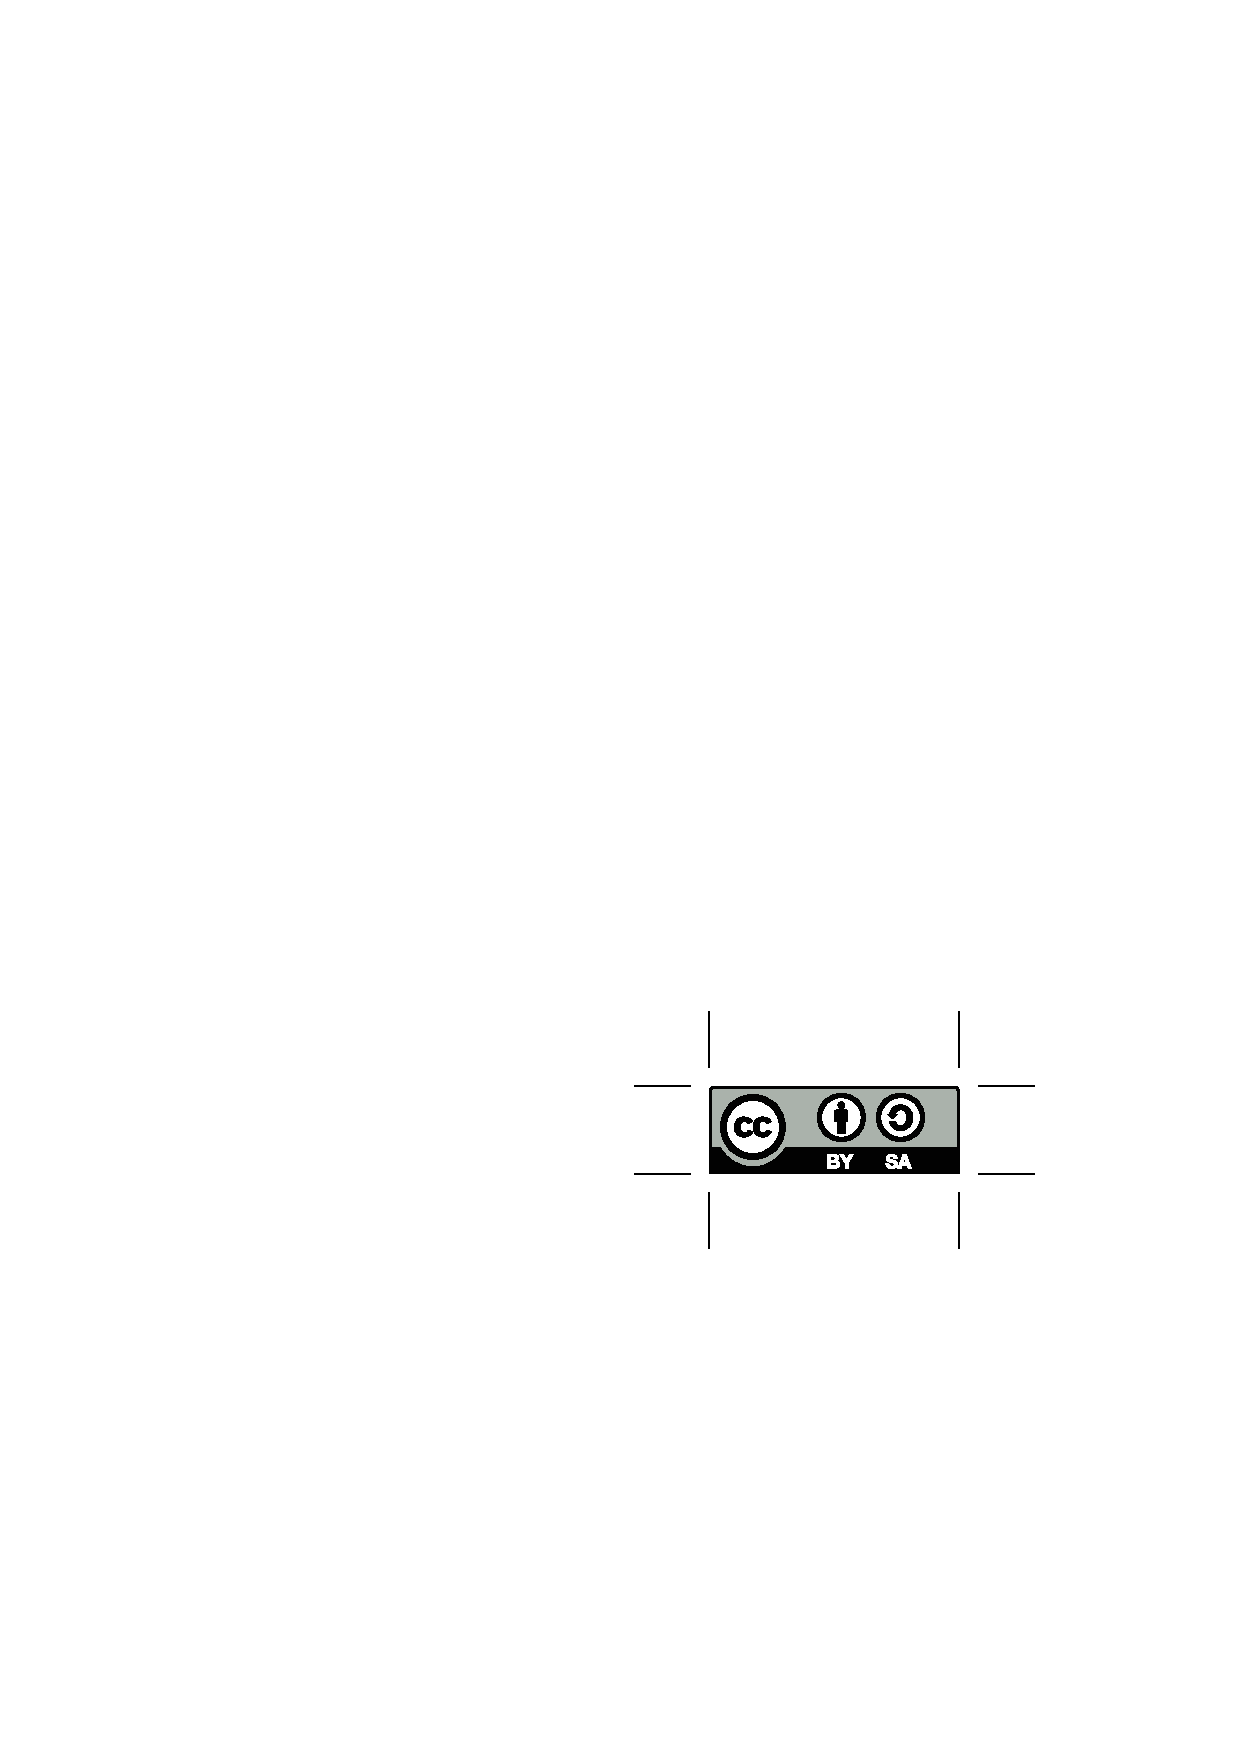
\includegraphics{cc-by-sa}

\noindent
This thesis is a free document.
You are able to distribute it under the terms of the license
Creative Commons - Attribution - Share Alike

\noindent
Aquesta tesi és un document lliure.
El podeu distribuir segons els termes de la llicència
Creative Commons - Atribució - Compartir en iguals condicions

\end{titlingpage}
\frontmatter

\cleartorecto % Comença a la pàgina dreta següent


%% Dedicatòria (opcional)
%% ------------------------------------------------------------
\thispagestyle{empty}
\vspace*{\stretch{1}}
\begin{flushright}
  \LARGE
  \itshape
Dedicatòria
\end{flushright}
\vspace*{\stretch{4}}

\cleartorecto

%% Acknowledgments
%% ------------------------------------------------------------
\chapter*{Acknowledgments}
\ldots

\cleartorecto
\cleartorecto
\thispagestyle{chapter}
\section*{Abstract}
\selectlanguage{english}
This is the abstract of the thesis in English.  Please, use less
than 150 words.

\selectlanguage{catalan}
\vspace*{\fill}
\section*{Resum}
Vet aquí el resum de la tesi en català.  Si us plau, utilitzeu
menys de 150 paraules.
\vspace*{\fill}

\cleartorecto

\pagestyle{headings}
%% Prefaci o pròleg
%% ---------------------------------------------------------------------- 
\chapter{Preface}
Introducció a la tesi que acostuma a ressenyar-ne els mèrits, el
valor, o també situar-la dins un context i unes circumstàncies
determinades.

\vspace{1cm}
Aquest document es pot descarregar de
\begin{quotation}
%\url{http://upf.edu/dtip/~autor/tesi.pdf}
\url{http://upf.edu/dtip/~autor/tesi.pdf}
\end{quotation}
\cleartorecto


\tableofcontents % presenta la taula de continguts
%\clearpage      % presenta la taula de figures
%\listoffigures
%\clearpage
%\listoftables   % presenta la taula de taules


%% Cos de la tesi
%% ---------------------------------------------------------------------
\mainmatter


\input{content}


\backmatter

\bibliographystyle{upfstyle} % 
\bibliography{../BinauralSynthesis} % el meu arxiu .bib de referències (sense
                        % extensió)
%% bibliografia
% En aquest cas, l'escrivim nosaltres a mà. En general és molt més
% convenient fer servir BibTeX.
%\begin{thebibliography}{tesi}
%  \bibitem[Gar66]{GARDNER66}
%    Martin Gardner.
%    \newblock \emph{More Mathematical Puzzles and Diversions}.
%    \newblock Penguin Books
%    \newblock (ISBN 0--14--020748--1), 1966.
%
%  \bibitem[GMS94]{GOOSSENS94}
%    Michel Goossens, Frank Mittelbach and Alexander Samarin.
%    \newblock \emph{The LaTeX Companion}.
%    \newblock Addison-Wesley Publishing Company
%    \newblock (ISBN 0--201--54199--8), 1994.
%
%  \bibitem[FAR85]{fary85}
%    José Luis Cantero Rada, \emph{El Fary}.
%    \newblock \emph{Yo detesto al hombre blandengue}
%    \newblock Entrevista a Televisió Espanyola,
%    octubre 1985.
%  \bibitem[ONS44]{onsager1944} Lars Onsager, \newblock
%    \emph{Crystal Statistics. I. A Two-Dimensional Model with an Order-Disorder Transition},
%    \newblock Physical Review \textbf{65}(3-4),
%    p 118--149, 1944.
%\end{thebibliography}

\clearpage

%% índex de noms
%\pagestyle{index}
%\printindex
%\cleardoublepage

\pagestyle{empty}
\null\vfil

%\begin{adjustwidth}{1in}{1in}
\begin{center}
{\Large Colophon}
\end{center}
\begin{center}
	Aquesta tesi s'ha escrit en \LaTeX\ fent servir l'editor
        \texttt{vim}.\\
	El cos de la lletra és XXX i a s'han utilitzat les fonts
	YYY.
\end{center}
%\end{adjustwidth}
\vfil

\end{document}
% vim:set tw=66:
